\section{Types of SPADs}\label{ssec:SPADs}
In Hazard Detection Mode, individual SPADs will have the responsibility of measuring their part in the target. Therefore it is important to first investigate what type of SPAD is best suited for the device. As mentioned in \cref{ssec:optics}, SPADs can have microlenses. Two types are considered: conventional spherical lenses, and rectangular lenses. Spherical lenses typically achieve an effective active area of approximately $55\,\%$, while rectangular lenses typically get an effective active area of appeoximately $65\,\%$. The active area can also be shaped in different sizes, and a circular and rectangular shape are considered here. An overview of the different options is shown in \cref{tkz:SPAD_types}.


\begin{figure}[H]
    \centering

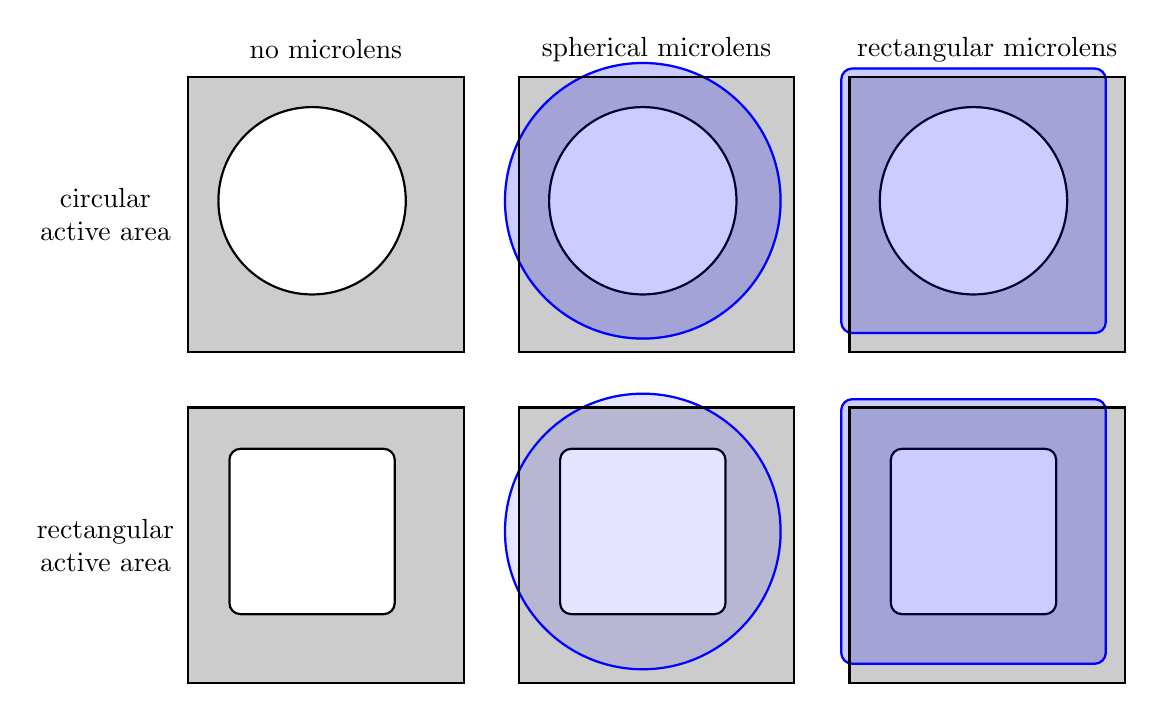
\begin{tikzpicture}[thick,scale=0.7, every node/.style={scale=1}]

\draw[fill, color=black!20]  (-1.25,3.25) rectangle (3.75,-1.75);
\draw[fill, color=white]  (1,1) ellipse (1.7 and 1.7);
\draw[]  (1,1) ellipse (1.7 and 1.7);

\draw[fill, color=black!20]  (4.75,3.25) rectangle (9.75,-1.75);
\draw[fill, color=white]  (7,1) ellipse (1.7 and 1.7);
\draw[]  (7,1) ellipse (1.7 and 1.7);
\draw [fill, color=blue, opacity=0.2] (7,1) ellipse (2.5 and 2.5);
\draw [color=blue] (7,1) ellipse (2.5 and 2.5);

\draw[fill, color=black!20]  (10.75,3.25) rectangle (15.75,-1.75);
\draw[fill, color=white]  (13,1) ellipse (1.7 and 1.7);
\draw[]  (13,1) ellipse (1.7 and 1.7);
\draw [fill, color=blue, opacity=0.2, rounded corners] (10.6,3.4) rectangle (15.4,-1.4);
\draw [color=blue, rounded corners] (10.6,3.4) rectangle (15.4,-1.4);

\draw[fill, color=black!20]  (-1.25,-2.75) rectangle (3.75,-7.75);
\draw[fill, color=white, rounded corners] (-0.5,-3.5) rectangle (2.5,-6.5) {};
\draw[rounded corners] (-0.5,-3.5) rectangle (2.5,-6.5) {};

\draw[fill, color=black!20]  (4.75,-2.75) rectangle (9.75,-7.75);
\draw[fill, color=white, rounded corners] (5.5,-3.5) rectangle (8.5,-6.5) {};
\draw[rounded corners] (5.5,-3.5) rectangle (8.5,-6.5) {};
\draw [fill, color=blue, opacity=0.1] (7,-5) ellipse (2.5 and 2.5);
\draw [color=blue] (7,-5) ellipse (2.5 and 2.5);

\draw[fill, color=black!20]  (10.75,-2.75) rectangle (15.75,-7.75);
\draw[fill, color=white, rounded corners] (11.5,-3.5) rectangle (14.5,-6.5) {};
\draw[rounded corners] (11.5,-3.5) rectangle (14.5,-6.5) {};
\draw [fill, color=blue, opacity=0.2, rounded corners] (10.6,-2.6) rectangle (15.4,-7.4);
\draw [color=blue, rounded corners] (10.6,-2.6) rectangle (15.4,-7.4);

\draw[]  (-1.25,3.25) rectangle (3.75,-1.75);
\draw[]  (4.75,3.25) rectangle (9.75,-1.75);
\draw[]  (10.75,3.25) rectangle (15.75,-1.75);

\draw[]  (-1.25,-2.75) rectangle (3.75,-7.75);
\draw[]  (4.75,-2.75) rectangle (9.75,-7.75);
\draw[]  (10.75,-2.75) rectangle (15.75,-7.75);

\node at (1.25,3.75) {no microlens};
\node at (7.25,3.75) {spherical microlens};
\node at (13.25,3.75) {rectangular microlens};
\node[align=center] at (-2.75,0.75) {circular\\active area};
\node[align=center] at (-2.75,-5.25) {rectangular\\active area};
\end{tikzpicture}
    \caption{Options for lenses with varying types of active areas and microlenses}
    \label{tkz:SPAD_types}
\end{figure}


The use of microlenses is not the only viable of option of increasing the active area on the chip. A second option is to pick the circuitry required per SPAD, and push it to the side. These circuitry include the Read-Out Integrated Circuit (ROIC) that also includes the quenching of the SPADs, and the Time interval to Digital converter (TDC). It is important to note that the push-out of the circuitry poses additional constraints of the design. The pushed out electronics must still be in a reasonable close range to the SPADs, which limits the dimensions of a device using push-out electronoics.

To avoid pileup, the following calculations are done for an $0.18\,\mu m$ technology and it is assumed that the ROIC will take up $110\,\mu m^2$ surface area per SPAD, and that the TDC will take up $1200\,\mu m^2$ surface area per SPAD. It will also be assumed that the minimum amount of pitch between two SPADs is $1.5\,\mu m$. These numbers are based on current SPAD designs in $0.18\,\mu m$ technology. An overview of the performance of all different possibilities is shown in \cref{fig:effective_area}. Note that, while the microlensen are assumed to focus the light on an arbitrarily small area, this is in reality not the case. If one would use no push-out electronics with a microlens for example, the pitch must be at least $40\,\mu m$ because otherwise there will not even be active area to focus the light on.

\begin{figure}[h]
\centering
	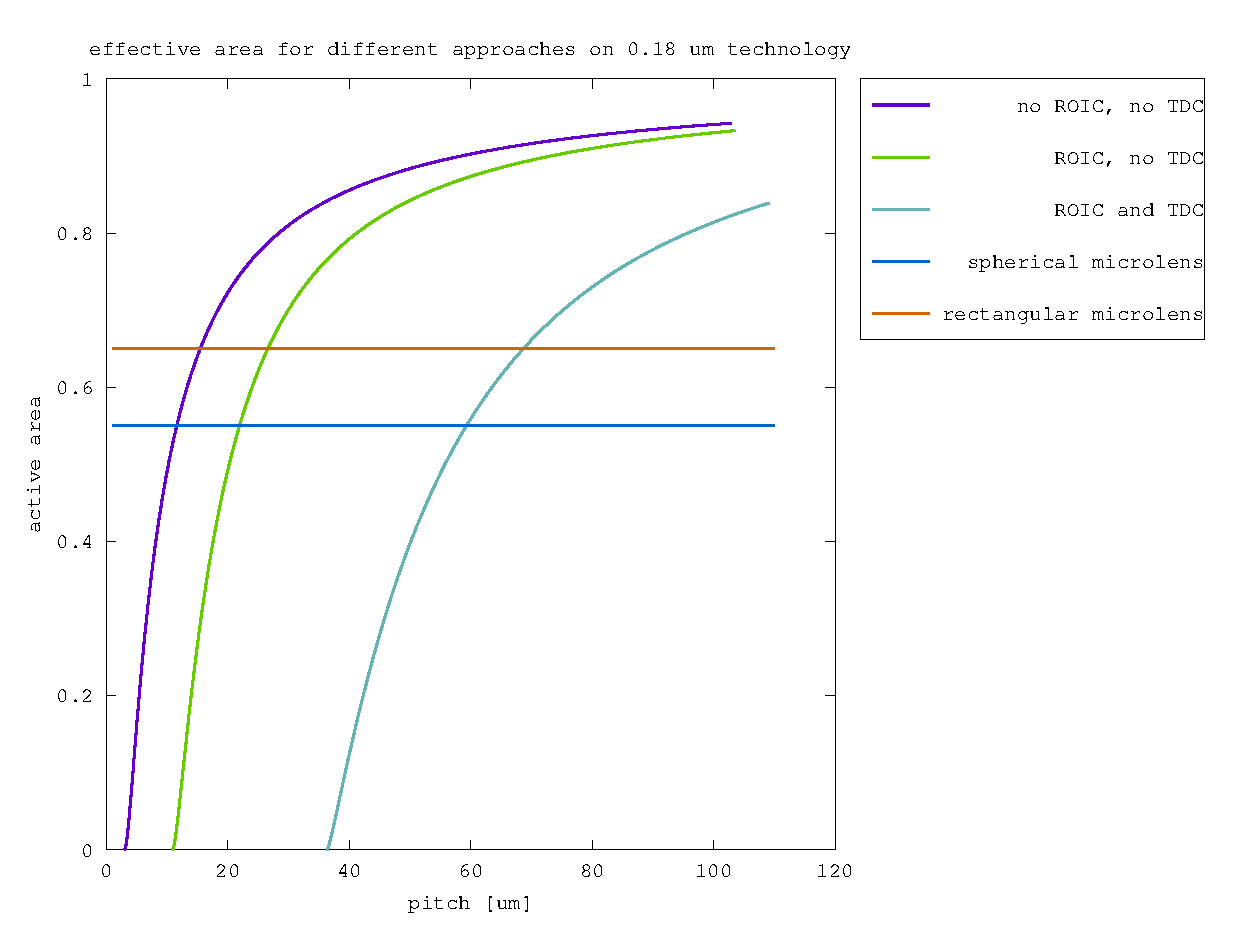
\includegraphics[width=0.8\linewidth]{fig/effective_area.eps}
\caption{Fillfactor for different approaches in relationship to the pitch of the SPAD on $0.18\,\mu m$ technology}
\label{fig:effective_area}
\end{figure} 

\section{Scanning motion}\label{ssec:scanning_motion}
The specifications indicate a target area of $125\times125\,m^2$ with a ground sample distance of $5\,cm$. This results in $2500\times2500$ pixels. For now however an array of $2048\times2048$ pixels will be considered, because that is a more convenient power of 2. 
Depending on the SPAD layout, different scanning motions arerequired to cover the target area. Possible scanning motions for different SPAD array configurations are shown in \cref{tkz:scanning_motions}. Note that the $2048\times1$ motion is in essense a special case of the $2048\times N$ motion, where exactly one row of pixels is observed at a time. $2048\times2048$ is also a special case of $2048\times N$ where no scanning motion is needed. The $M\times N$, with $M<2048$ and $N<2048$ needs a scanning motion in both x and y direction. This makes the scanning motion very complicated and unreliable. Therefore only the family of solutions with $2048\times N$ will be considered.


\begin{figure}[H]
    \centering
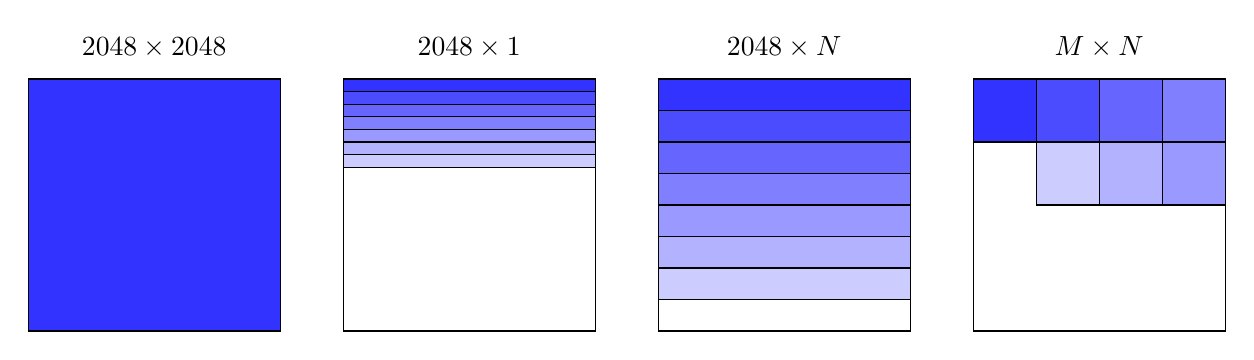
\begin{tikzpicture}[scale=.8]
\draw  (-3,4) rectangle (1,0);
\draw [fill=blue!80] (-3,4) rectangle (1,3.8);
\draw [fill=blue!70] (-3,3.8) rectangle (1,3.6);
\draw [fill=blue!60] (-3,3.6) rectangle (1,3.4);
\draw [fill=blue!50] (-3,3.4) rectangle (1,3.2);
\draw [fill=blue!40] (-3,3.2) rectangle (1,3);
\draw [fill=blue!30] (-3,3) rectangle (1,2.8);
\draw [fill=blue!20] (-3,2.8) rectangle (1,2.6);


\draw  (2,4) rectangle (6,0);
\draw [fill=blue!80] (2,4) rectangle (6,3.5);
\draw [fill=blue!70] (2,3.5) rectangle (6,3);
\draw [fill=blue!60] (2,3) rectangle (6,2.5);
\draw [fill=blue!50] (2,2.5) rectangle (6,2);
\draw [fill=blue!40] (2,2) rectangle (6,1.5);
\draw [fill=blue!30] (2,1.5) rectangle (6,1);
\draw [fill=blue!20] (2,1) rectangle (6,0.5);


\draw  (7,4) rectangle (11,0);
\draw [fill=blue!80] (7,4) rectangle (8,3);
\draw [fill=blue!70] (8,4) rectangle (9,3);
\draw [fill=blue!60] (9,4) rectangle (10,3);
\draw [fill=blue!50] (10,4) rectangle (11,3);
\draw [fill=blue!40] (10,3) rectangle (11,2);
\draw [fill=blue!30] (9,3) rectangle (10,2);
\draw [fill=blue!20] (8,3) rectangle (9,2);

\node at (-6,4.5) {$2048\times2048$};
\node at (-1,4.5) {$2048\times1$};
\node at (4,4.5) {$2048\times N$};
\node at (9,4.5) {$M\times N$};

\draw [fill=blue!80] (-8,4) rectangle (-4,0);
\end{tikzpicture}
    \caption{Different types of scanning motions}
    \label{tkz:scanning_motions}
\end{figure}
\section{SPAD layout}\label{ssec:SPAD_layout}
The results in \cref{fig:effective_area} clearly show that an increase in the pitch will also increase the part of the SPAD that is active. However, arbitrarily large pitches cannot be afforded. An array of $2048\times2048$ does not allow for push-out electronics. Therefore the minimum pitch is $40\,mu m$ combined with a microlens. This amount of pixels would result in a chip area of $8\times8\,cm^2$ which is not feasable with current manufacturing technology. This means that with current technology constraints a $2048\times2048$ SPAD array cannot be manufactured and is therefore not feasable. In fact, even in a single dimension, $8\,cm$ is not feasable. This means that push-out electronics of at least the TDC are a requirement to meet the pixel density requirements.

The push-out electronics pose a restriction that the electronics must be at most 4, or in extreme cases, 8 SPAD pitches away from the SPAD. This restricts the SPAD array to a maximum of $2048\times8$  pixels. To avoid pileup, only the feasability of a pitch of $20\,\mu m$ will be investigated. Using the results obtained in \cref{fig:effective_area}, one can see that the effectiveness of a SPAD with push-out ROIC is approximately $75\,\%$ and the effectiveness of a SPAD with onboard ROIC approximately $55\,\%$. The surface area of the SPAD array is a line with a length of $4\,cm$ and a width of atleast $160\,\mu m$. There is no point in using microlenses for these dimensions. They add little to no benefit on the efficiency, and there are several issues with the use of microlenses, like restrictions on the lens, that can't make them justifiable in this setup. To avoid pileup, the feasbility of a SPAD array of $2048\times8$ will be considered.
